
\documentclass[11 pt]{article}
\usepackage[top=1in, bottom=1in, left=0.5in, right=0.5in]{geometry}
\usepackage{graphicx}
\usepackage{amsmath}
\usepackage{natbib}
\begin{document}
\title{Physics Behind the Simulation: A CS296 Report by Group 25}
\author{ Amal Dani\\
  \texttt{120020019}\\
  \texttt{amaldani@iitb.ac.in}
  \and
         Manohar Kumar\\
  \texttt{120050044}\\
  \texttt{mano1994@iitb.ac.in}}
\date{22, January 2014}
\maketitle
\section{Introduction}
This is an article written to explain the three mobile objects that has been added to the CS296 BASE CODE. It briefly describes the physics behind it and gives a slight mathematical insight. It tries to express the utility of BOX2D\cite{box2d} in the field of 2D simulation of machines where the Newtonian Physics holds.
\section{Physics behind the simulation.}
This section describes the three objects added by us in the code. They are a ROLLING sphere, TOPPLING octagon, MOVABLE inclined plane. I must accept all these objects are manifestations of the objects used in problems of Mechanics in JEE Physics.
\subsection{ROLLING SPHERE}
The sphere is given a non zero friction coefficient, hence it rolls. It is initially at state of rest when a sphere of much larger mass strikes it. It is a head on collision, and there is a transfer of energy, such that the conservation of momentum holds. We also apply the conservation of Kinetic Energy on the system to reach a conclusion on final velocities. The rolling takes place because of non zero coefficient of friction\cite{hrk}. This is due to the rotation produced due to the unbalanced torque on the ball. The ball follows its way to the inclined plane.
\begin{center}
\includegraphics[width=7cm, height=7cm]{sphere.eps}\end{center}
\begin{equation} \: \frac{Mv_{Mi}^{2}}{2} \: =  \: \frac{Mv_{Mf}^{2}}{2} \: +  \: \frac{mv_{mf}^{2}}{2} \:  \end{equation}
\begin{equation} \: {Mv_{Mi}^{2}} \: =  \: {Mv_{Mf}^{2}} \: +  \: {mv_{mf}^{2}} \:  \end{equation}
\begin{equation} \: \beta mg \: = \: Ir \alpha \: \end{equation}
\begin{itemize}
\item $M(kg)=$ Mass of the heavier non rolling sphere 
\item $m(kg)=$ Mass of the lighter rolling sphere  
\item $v_{mi}(m/s)$=initial velocity of body of mass $m$ 
\item $v_{Mi}(m/s)$=initial velocity of body of mass $M$
\item $v_{mf}(m/s)$=final velocity of body of mass $m$ 
\item $v_{Mf}(m/s)$=final velocity of body of mass $M$ 
\item $\beta$=coefficient of friction of collision of body of mass m 
\item $g(m/s^{2})$=acceleration due to gravity 
\item $I(kg.m^{2})$=Moment of Inertia of body of mass m 
\item $r(m)$=radius of the body of mass m 
\item $\alpha(rad/s^{2})$=angular accelaration of the body of mass m
\end{itemize}


\subsection{INCLINED PLANE}
It is a moving plane. It implies it has finite mass. Now the heading sphere collides with the inclined plane, as the mass of the rolling sphere is extremely small, the inclined plane hardly moves. The impact is mainly from the heavier non-rolling sphere that is following. The velocity of the plane post collision can be calculated by conservation of momentum and as the coefficient of restitution of the plane is zero, the velocity of both the inclined plane and the non rolling sphere is the same post collision.\cite{hcv} This is evident from the equation of restitution. The motion of the sphere perpendicular to the inclined plane is zero relative to the inclined.
\begin{center}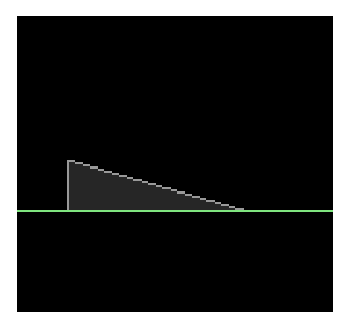
\includegraphics[width=7cm, height=7cm]{inclined.eps}\end{center}
\begin{equation} N \: + \: m a_{p} sin \theta \: = \: m g \: cos \theta \end{equation}
\begin{itemize}
\item $m(kg)=$ Mass of the lighter rolling sphere   
\item $g(m/s^{2})$=acceleration due to gravity 
\item $\theta(rad)$= angle of the incline plane 
\item $a_{p}(m/s^{2})$= pseudo acceleration due to motion of the inclined plane
\item $N(Newton)$= Normal force acting on the sphere due to contact with the inclined 
\end{itemize}

\subsection{TOPPLING OCTAGON}
The octagon is a relatively light object to facilitate motion. Toppling is also facilitated by its relatively smaller edge length in contact with the surface \cite{hcv}. The moving inclined plane strikes it at a height such that the torque applied by the impact is greater than the maximum torque that could be provided to maintain stability\cite{hrk}. Hence the octagon topples. When in motion it has friction too.When the impact is faced the friction tries to oppose the motion of the point of contact. If the maximum kinetic friction possible is unable to balance the impact of torque the object topples.\cite{hrk}
\begin{center}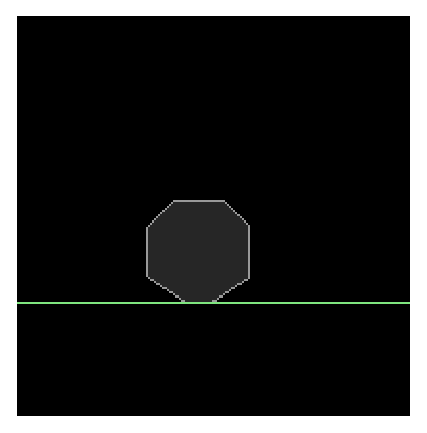
\includegraphics[width=7cm, height=7cm]{octagon.eps}\end{center}
\begin{equation}F d_{1} \: - \beta N d_{2}\:= \:Id_{2} \alpha \end{equation}
\begin{itemize}
\item $F(Newton)$=Impact force due to collision 
\item $d_{1}(m)$=Perpendicular distance between line of force and horizonal line passing through centre 
\item $d_{2}(m)$=Perpendicular distance between line of friction and horizonal line passing through centre 
\item $\beta$ =coefficient of friction of collision of body of octagon
\item $N(Newton)$=Normal force acting on octagon 
\item $I(kgm^{2})$=Moment of inertia of octagon 
\item $\alpha(rad/s^{2})$=angular acceleration of the octagon when toppled 
\end{itemize}

\section{Conclusions}
We have analysed the three addition to the BOX2D Base Code, and mentioned the physics behind it. We have mainly covered the Newtonian Mechanics. Conservation of Momentum and Rotational Dynamics is the crux of the article.

\bibliographystyle{plain}
\bibliography{references}

  
\end{document}



